% GNUPLOT: LaTeX picture with Postscript
\begingroup
  \makeatletter
  \providecommand\color[2][]{%
    \GenericError{(gnuplot) \space\space\space\@spaces}{%
      Package color not loaded in conjunction with
      terminal option `colourtext'%
    }{See the gnuplot documentation for explanation.%
    }{Either use 'blacktext' in gnuplot or load the package
      color.sty in LaTeX.}%
    \renewcommand\color[2][]{}%
  }%
  \providecommand\includegraphics[2][]{%
    \GenericError{(gnuplot) \space\space\space\@spaces}{%
      Package graphicx or graphics not loaded%
    }{See the gnuplot documentation for explanation.%
    }{The gnuplot epslatex terminal needs graphicx.sty or graphics.sty.}%
    \renewcommand\includegraphics[2][]{}%
  }%
  \providecommand\rotatebox[2]{#2}%
  \@ifundefined{ifGPcolor}{%
    \newif\ifGPcolor
    \GPcolortrue
  }{}%
  \@ifundefined{ifGPblacktext}{%
    \newif\ifGPblacktext
    \GPblacktextfalse
  }{}%
  % define a \g@addto@macro without @ in the name:
  \let\gplgaddtomacro\g@addto@macro
  % define empty templates for all commands taking text:
  \gdef\gplbacktext{}%
  \gdef\gplfronttext{}%
  \makeatother
  \ifGPblacktext
    % no textcolor at all
    \def\colorrgb#1{}%
    \def\colorgray#1{}%
  \else
    % gray or color?
    \ifGPcolor
      \def\colorrgb#1{\color[rgb]{#1}}%
      \def\colorgray#1{\color[gray]{#1}}%
      \expandafter\def\csname LTw\endcsname{\color{white}}%
      \expandafter\def\csname LTb\endcsname{\color{black}}%
      \expandafter\def\csname LTa\endcsname{\color{black}}%
      \expandafter\def\csname LT0\endcsname{\color[rgb]{1,0,0}}%
      \expandafter\def\csname LT1\endcsname{\color[rgb]{0,1,0}}%
      \expandafter\def\csname LT2\endcsname{\color[rgb]{0,0,1}}%
      \expandafter\def\csname LT3\endcsname{\color[rgb]{1,0,1}}%
      \expandafter\def\csname LT4\endcsname{\color[rgb]{0,1,1}}%
      \expandafter\def\csname LT5\endcsname{\color[rgb]{1,1,0}}%
      \expandafter\def\csname LT6\endcsname{\color[rgb]{0,0,0}}%
      \expandafter\def\csname LT7\endcsname{\color[rgb]{1,0.3,0}}%
      \expandafter\def\csname LT8\endcsname{\color[rgb]{0.5,0.5,0.5}}%
    \else
      % gray
      \def\colorrgb#1{\color{black}}%
      \def\colorgray#1{\color[gray]{#1}}%
      \expandafter\def\csname LTw\endcsname{\color{white}}%
      \expandafter\def\csname LTb\endcsname{\color{black}}%
      \expandafter\def\csname LTa\endcsname{\color{black}}%
      \expandafter\def\csname LT0\endcsname{\color{black}}%
      \expandafter\def\csname LT1\endcsname{\color{black}}%
      \expandafter\def\csname LT2\endcsname{\color{black}}%
      \expandafter\def\csname LT3\endcsname{\color{black}}%
      \expandafter\def\csname LT4\endcsname{\color{black}}%
      \expandafter\def\csname LT5\endcsname{\color{black}}%
      \expandafter\def\csname LT6\endcsname{\color{black}}%
      \expandafter\def\csname LT7\endcsname{\color{black}}%
      \expandafter\def\csname LT8\endcsname{\color{black}}%
    \fi
  \fi
  \setlength{\unitlength}{0.0500bp}%
  \begin{picture}(9636.00,5668.00)%
    \gplgaddtomacro\gplbacktext{%
      \csname LTb\endcsname%
      \put(814,704){\makebox(0,0)[r]{\strut{} 0}}%
      \csname LTb\endcsname%
      \put(814,1487){\makebox(0,0)[r]{\strut{} 10}}%
      \csname LTb\endcsname%
      \put(814,2270){\makebox(0,0)[r]{\strut{} 20}}%
      \csname LTb\endcsname%
      \put(814,3054){\makebox(0,0)[r]{\strut{} 30}}%
      \csname LTb\endcsname%
      \put(814,3837){\makebox(0,0)[r]{\strut{} 40}}%
      \csname LTb\endcsname%
      \put(814,4620){\makebox(0,0)[r]{\strut{} 50}}%
      \csname LTb\endcsname%
      \put(814,5403){\makebox(0,0)[r]{\strut{} 60}}%
      \csname LTb\endcsname%
      \put(1700,484){\makebox(0,0){\strut{}2A}}%
      \csname LTb\endcsname%
      \put(2454,484){\makebox(0,0){\strut{}2B}}%
      \csname LTb\endcsname%
      \put(3208,484){\makebox(0,0){\strut{}2C}}%
      \csname LTb\endcsname%
      \put(3962,484){\makebox(0,0){\strut{}3A}}%
      \csname LTb\endcsname%
      \put(4716,484){\makebox(0,0){\strut{}3B1}}%
      \csname LTb\endcsname%
      \put(5469,484){\makebox(0,0){\strut{}3B2}}%
      \csname LTb\endcsname%
      \put(6223,484){\makebox(0,0){\strut{}3B3}}%
      \csname LTb\endcsname%
      \put(6977,484){\makebox(0,0){\strut{}3B4}}%
      \csname LTb\endcsname%
      \put(7731,484){\makebox(0,0){\strut{}3C}}%
      \csname LTb\endcsname%
      \put(8485,484){\makebox(0,0){\strut{}3D}}%
      \put(176,3053){\rotatebox{-270}{\makebox(0,0){\strut{}PSNR (dB)}}}%
      \put(5092,154){\makebox(0,0){\strut{}Exercise}}%
    }%
    \gplgaddtomacro\gplfronttext{%
      \csname LTb\endcsname%
      \put(8252,5230){\makebox(0,0)[r]{\strut{}Beowulf Simple}}%
      \csname LTb\endcsname%
      \put(8252,5010){\makebox(0,0)[r]{\strut{}Elephants Dream Simple}}%
      \csname LTb\endcsname%
      \put(8252,4790){\makebox(0,0)[r]{\strut{}The Seeker Dark Rising Simple}}%
      \csname LTb\endcsname%
      \put(8252,4570){\makebox(0,0)[r]{\strut{}Beowulf Complex}}%
      \csname LTb\endcsname%
      \put(8252,4350){\makebox(0,0)[r]{\strut{}Elephants Dream Complex}}%
      \csname LTb\endcsname%
      \put(8252,4130){\makebox(0,0)[r]{\strut{}The Seeker Dark Rising Complex}}%
    }%
    \gplbacktext
    \put(0,0){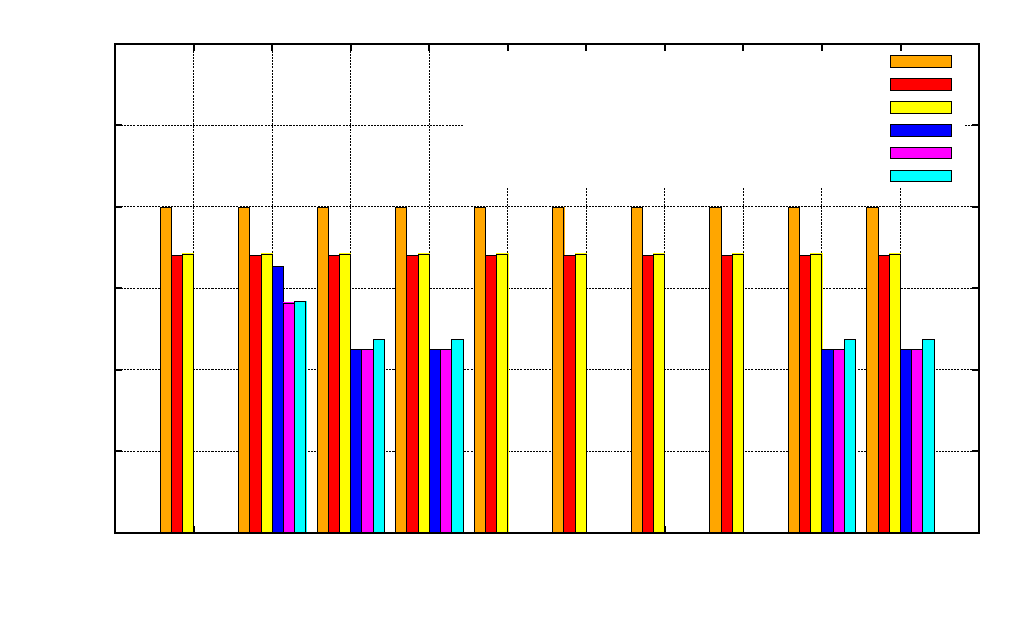
\includegraphics{psnr}}%
    \gplfronttext
  \end{picture}%
\endgroup
